\documentclass[]{beamer}
%for printing or having a crappy pdf reader backup
%\documentclass[handout]{beamer}
\mode<presentation>
\usetheme{Madrid}


\usecolortheme[RGB={80,0,0}]{structure}
%teal \usecolortheme[RGB={0,128,128}]{structure}
\useoutertheme{miniframes}
\useinnertheme{default}
\usepackage{color}
\definecolor{Maroon}{RGB}{80,0,0}
\definecolor{BurntOrange}{RGB}{204,85,0}
\usepackage{setspace}
\usepackage{amsmath}
\usepackage{amsthm}
\usepackage{amsfonts}
\usepackage{amssymb}
\usepackage{verbatim}
\usepackage{array}
\usepackage{graphicx}
\usepackage{subfigure}
\usepackage{colortbl}
%\usepackage[retainorgcmds]{IEEEtrantools}
\usepackage{wrapfig}
\usepackage[figurename=,tablename=]{caption}
\usepackage{multirow}
\setbeamercolor{normal text}{fg=black}
\setbeamercovered{dynamic}
\beamertemplatetransparentcovereddynamicmedium
%\usepackage{chronology}
\setbeamertemplate{caption}[numbered]
\usepackage{colortbl}
\newcommand {\mathsym}[1]{{}}
\newcommand {\unicode}{{}}
\newcommand{\om}{\boldsymbol{\Omega}}
\newcommand{\etal}{{\it et al.\,}}
\newcommand{\vr}{\vec{r}}
\newcommand{\vo}{\vec{\Omega}}
\newcolumntype{L}{>{\centering\arraybackslash}m{3cm}}
\newcommand{\tcr}[1]{\textcolor{red}{#1}}
%Creating a norm command
\newcommand{\norm}[1]{\left\lVert#1\right\rVert}
%Allow page breaks within align
\allowdisplaybreaks
%Code
\usepackage{listings}
\usepackage{pdfpages}
\newlength \figwidth
\setlength \figwidth {0.5\textwidth}

\usepackage[percent]{overpic}



\begin{document}
%	

\title[XFEM Moving Interface Verification]{Extended Finite Element Method Development \& Application for Simulation of Moving Interface \& Boundary Phenomena}
\author[Tompkins]{James B. Tompkins \\ Chair: Dr. Ryan G. McClarren \\ Co-chair: Dr. Jean C. Ragusa \\ Committee: Drs. J.N. Reddy \& Lin Shao}
\institute[TAMU]{Texas A\&M University}
%\committee[McClarren,Arroyave,Ragusa,Shao,Hales]{Dr. Ryan McClarren \\ Dr. Raymundo Arr\'{o}yave \\ Dr. Jean Ragusa \\ Dr. Lin Shao \\ Dr. Jason Hales}
\date[Sept 6, 2018]

% ###############################################################################
\section{2D RZ LS Dep}
\subsection{}
% ###############################################################################
\begin{frame}[t]\frametitle{2D, Cylindrical, Level Set Dependent Material Problem Description}
  \begin{block}{PDE}
    $\rho c_p\frac{\partial T}{\partial t} - \nabla k \nabla T = 
    \rho c_p\frac{\partial T}{\partial t} - \frac{1}{r}\frac{\partial}{\partial r}
    \left(r\cdot k\frac{\partial T}{\partial r}\right) - \frac{\partial}{\partial z}
    \left(k\frac{\partial T}{\partial z}\right)= q$
  \end{block}
  
  \begin{block}{Advection PDE for Level Set}
    $\frac{\partial \phi}{\partial t} + u(r,z,t) \cdot \nabla \phi = 0 \; , \; 
    \frac{\partial \phi}{\partial t} + u(r,z,t) \cdot \left( \frac{\partial \phi}
    {\partial r} + \frac{\partial \phi}{\partial z}\right) = 0$
  \end{block}
  
  \begin{block}{Domain/Material Properties}
  	$[\Omega_r,\Omega_z] = [[1,2],[1,2]]$ \\
  	$\rho cs_p = 10$ \\
  	$k(r,z,t) = \left(\frac{0.05}{2.04}\right) \phi(r,z,t) + 1.5$
  \end{block}
\end{frame}

\begin{frame}[t]\frametitle{2D, Cylindrical, Level Set Dependent Material Problem BCs/IC}
  \begin{block}{BCs}
    Left: \textbf{Neumann} -- $\left. \frac{\partial T}{\partial r}\right|_{r=1} = k(r,z,t)\cdot 100t$ \\
    Right: \textbf{Dirichlet} -- $T(2,z,t) = (-100z + 200)t +400$ \\
    Bottom: \textbf{Neumann} -- $\left. \frac{\partial T}{\partial z}\right|_{z=1} = k(r,z,t)\cdot 100t$ \\
    Top: \textbf{Dirichlet} -- $T(r,2,t) = (-100r + 200)t + 400$
  \end{block}
  
  \begin{block}{ICs}
    \textbf{Constant} -- $T(r,z,0) = 400$ \\
    \textbf{Function} -- $\phi(r,z,0) = -0.5(x+y) + 1.7$
  \end{block}
\end{frame}

\begin{frame}[t]\frametitle{Provided PDE Terms}
%  \begin{block}{Prescribed $T$ Solution}
%    $T(x,t) = (-100r-100z+400)t + 400$
%  \end{block}
  
  \begin{block}{Provided $T$ Source}
  $q = 100\,\rho c_p \left(-r-z+4\right)+ t\left(-\frac{2.5}{2.04}\frac{z}{r} + 155\frac{1}{r}
  +\frac{1}{2.04}\frac{t}{r} - \frac{7.5}{2.04}\right)$
  \end{block}
  
%  \begin{block}{Prescribed $\phi$ Interface Level Set Solution (\& $\phi$ Initial Condition)}
%    $\phi(x,y,t) = -0.5(x+y) + 2.04 - 0.2t$
%  \end{block}
  
  \begin{block}{Provided $\phi$ velocity term, $u(r,z,t)$}
    $u(r,z,t) = -\frac{0.07}{200} \left( T-410\right)-0.2$
  \end{block}
  
  \begin{block}{Note about Problem}
    This is a problem that fully couples the $T$ and $\phi$ solutions: $k$ is dependent on 
    $\phi$, and $u(r,z,t)$ is dependent on $T$. We have provided values to make the problem
    similar to previous MMS Verification problems, but still need to develop a version of
    this problem with an analytical solution in mind. This acts as more of a \textit{proof of 
    concept} than true verification problem.
  \end{block}
\end{frame}

%\begin{frame}\frametitle{Numerical Parameters}
%  	\begin{columns}
%		\column{0.32\linewidth}
%			\begin{center}
%			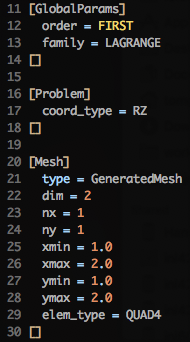
\includegraphics[scale=0.4]{figures/Screen-GlobalParams-2Drzls1m}
%			\end{center}
%		\column{0.66\linewidth}
%			\begin{center}
%			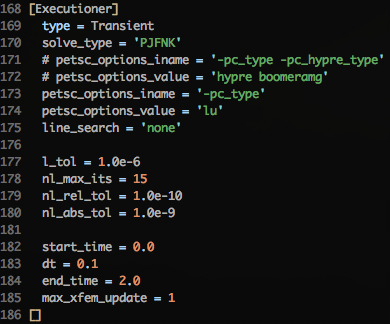
\includegraphics[scale=0.4]{figures/Screen-Executioner-2Drzls1m}
%			\end{center}
%	\end{columns}
%	\begin{center}
%	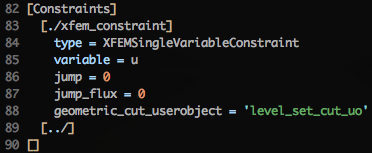
\includegraphics[scale=0.4]{figures/Screen-Constraints-2Drzls1m}
%	\end{center}
%\end{frame}

%\begin{frame}[t]\frametitle{$\phi$ Solution L2 Error Norms at Each Timestep}
%	\begin{center}
%		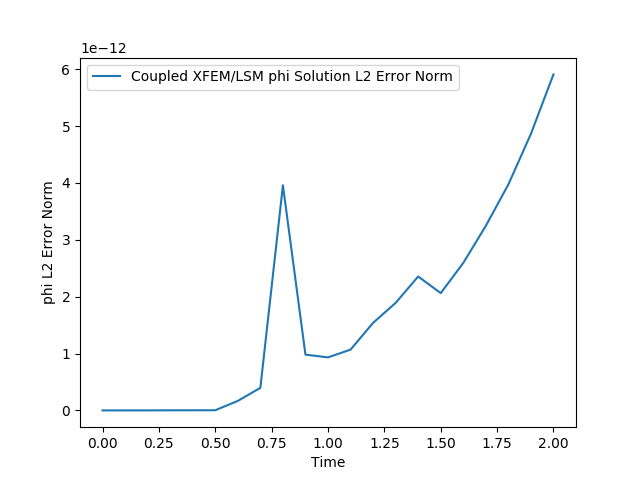
\includegraphics[scale=0.5]{figures/ls-xfem-2D_rz_ls1mat_phi_L2_Errs}
%	\end{center}
%\end{frame}
%
%\begin{frame}[t]\frametitle{$T$ Solution L2 Error Norms at Each Timestep}
%	\begin{center}
%		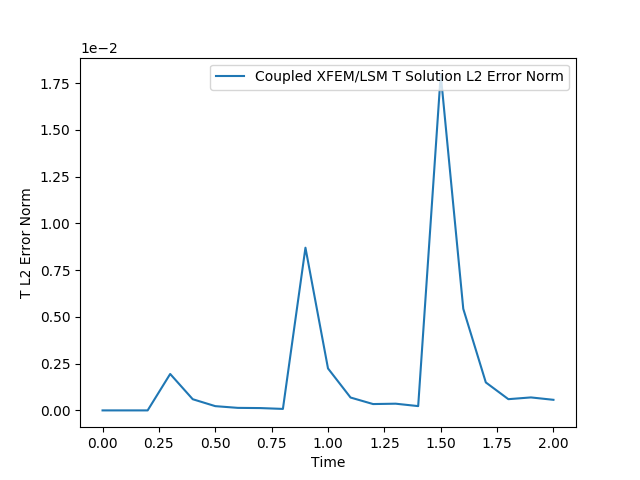
\includegraphics[scale=0.5]{figures/ls-xfem-2D_rz_ls1mat_u_L2_Errs}
%	\end{center}
%\end{frame}

\end{document}

%%% Slide template
%\begin{frame}[t]\frametitle{}
%% Slide Goal: 
%% Notes: 
%  \begin{block}{}
%
%  \end{block}
%\end{frame}
